\section{Single-Task Feed-forward Neural Networks} \label{sec:singletaskNN}
% TODO: citations!
% TODO: check nn math 
\emph{Feed-forward neural networks} (FNN), also known as multilayer perceptron, are artificial neural networks (ANN) that do not contain cycles. Despite the fact that many ANN models have failed the original attempts to reproduce the real structure of the brain mathematically, they became an efficient model for pattern recognition. 

Given a set $V$ of vertices and a set  $E\subseteq V\times V$ of edges, a feedforward neural network is described by a directed acyclic graph, $G =
(V,E)$, and a weight function over the edges, $w : E \to \mathbf R$ ($w(i, j) = 0$
for every $(i, j) \notin E$). The nodes of the graph correspond to neurons. Each
single neuron includes an \emph{activation function},  $ \sigma : \mathbf R \to
\mathbf R$. FNNs are usually
split in layers, that, is the nodes in $V$ are decomposed in disjoint sets $V_t$, $0\leq t\leq T$,
and $V = \cup_{t = 0}^T V_t$. $V_0$ and
$V_T$ are respectively called input and output layer; note that $|V_0| = d$ and
$|V_T| = n$ where $d$ is the dimensionality of the input space and $n$ the
dimensionality of the output space. Given the graph $G$, the map $w$ and the
activation function $\sigma$, the network is able to calculate the function
$f_{G,W,\sigma}$. For every node $i \in V$ a value $v_i$ is associated. Given $j
\in V \setminus V_0$, for every $(i, j) \in E$ we define $w(j)$, the vector containing all
the weights $w(i, j)$ and $v(j)$, the vector whose components are the values $v_i$. Now the
vector $f(x)$ is computed as follow:
\begin{enumerate}
    \item $v_i = x_i$ for every node $i \in V_0$;
    \item $v_j = \sigma(w(j)^T v(j))$ for every node $j \in V \setminus V_0$;
    \item $f_k = v_k$, where k is the $k$th output node.
\end{enumerate}
In Figure~\ref{fig:neural_network_example} we show an example of neural network architecture \cite{ShwartzUnderstadningML, BishopML}.
\begin{figure}[ht]
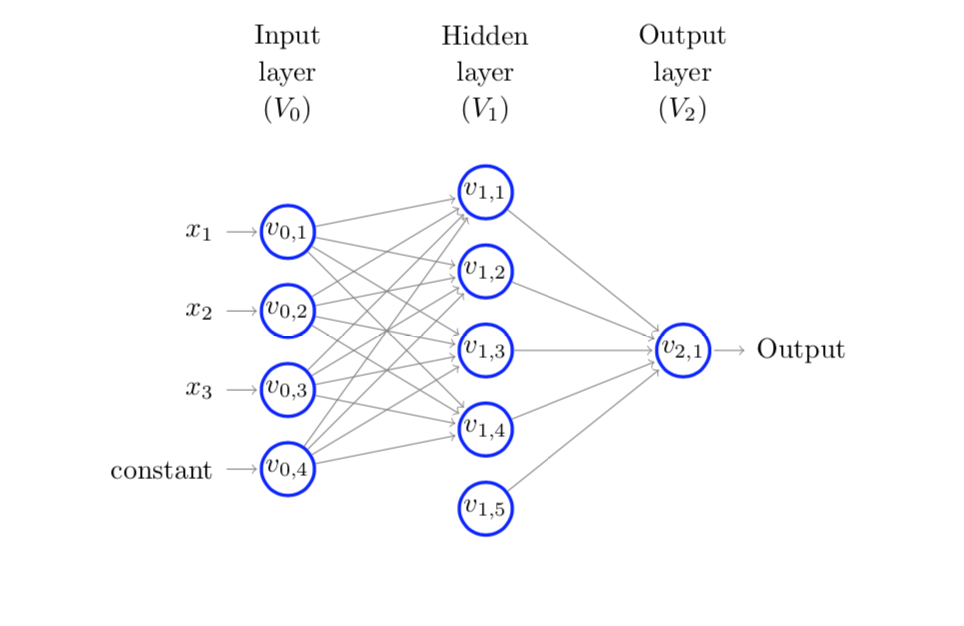
\includegraphics[width=\textwidth]{neural_network_example.png}
\caption{Neural Network architecture example, it has a 3-dimensional input layer
($V_0$), one hidden layer ($V_1$) and a single neuron output layer ($V_2$)
\cite{ShwartzUnderstadningML}.} 
\label{fig:neural_network_example}
\end{figure}

Starting from the tuple $(G, \sigma)$, often called the \emph{architecture of the network}, we can define the class of predictors: 
\[ \mathcal{F}_{G, \sigma} = \{ f_{G, \sigma, w} \mid w \textrm{ is a mapping from } E \textrm{ to } \mathbf R \} \]
From an expressiveness standpoint, it is proved that with a FNN using a binary input $x \in \{-1, 1\}^d$ and $\mathrm{sign}$ as activation
function $\sigma$, a single hidden layer network is able to
implement every binary function $f: \{-1, +1\}^d \to \{-1, +1\}$. Note that in practical term the binary constraint is just a useful simplification because a bit string of length $b$ represents every real coordinate in a computer.  That is, a single hidden layer is
enough to represent every Boolean function. The downside is that
the number of neurons required must be exponential in the dimension
of the input space. Currently, there are no mathematical proofs about the construction of
best network architecture for a given problem, nevertheless there is empirical evidence
about the fact that is better a network with fewer neurons distributed in many layers (deep
learning) rather than many neurons in a single layer. % TODO: citations

To train the weights of a feed-forward neural network is usually
used a gradient descent algorithm. The most commonly is called
Stochastic Gradient Descent (SGD). For every randomly sampled
example $x_t$ from the training set, the parameters $w(i, j)$ of the
network are updated using the following rule:
\begin{equation} \label{eq:sgd} 
w(i, j) \leftarrow w(i, j) -  \eta_t \frac{\delta\ell_{x_t}(W)}{\delta w(i, j )}
\end{equation}
where $\ell_(.)$ is a convex loss function. SGD is not the only
gradient descent algorithm used. In fact, in order to
improve the convergence of the neural networks many others algorithms were introduced,
the most popular were \emph{mini-batch gradient descent}, \emph{nesterov}, \emph{adagrad}
\cite{RuderGDOpt}. 

An algorithm called \emph{back-propagation} is used to compute the
gradients of the losses with respect of the weights in SGD. Using the chain rule of derivation the algorithm compute the gradient with a layer by layer backward iteration
\cite{HintonBackProp}.
 

\section{Multi-Task Neural Networks}\label{sec:MTLsection}
%TODO: soft and hard parameter sharing figures
Multi-Task learning (MTL) is becoming increasingly popular in recent years.
Usually, to optimizing the predictions of a given task, a single model is
tuned and trained. In this way, good results can be achieved but, any
information that might come from related tasks are lost. MTL methods take
the signal from related considered tasks by sharing the
representation between them. The typical setting is to learning simultaneously multiple
tasks using a shared representation, what is learned by one
task can be helpful for the other tasks and vice versa \cite{Caruana97}. 
The mechanism underlining MTL, firstly described by \cite{Caruana97}, are reported in this Section.
There are many motivation behind MTL: from a biological point of view is
inspired by the way the human brain learns (the knowledge of tasks can help us
learning other tasks), from a pure machine learning perspective
can be seen as a form of regularization in which the inductive bias is
introduced by the auxiliary tasks \cite{Ruder2017}. 

Multi-tasks learning introduces an \emph{implicit data augmentation}, that is, increase the sample size used to train the model. Furthermore, defining A and B as two related tasks with noise, learning A and B jointly gives a better representation due to the noise patterns averaging.
Also, MTL permits the model to \emph{focus attention} on the feature that really matters. This behaviour, considered as an implicit feature selection, is possible because other tasks could give additional evidence about relevance (or irrelevance) of features. 

MTL introduces the concept of \emph{eavesdropping}. The idea, introduced using hints by \cite{AbuMostafa1990}, is that we can allow the model to learn a features subset G, that is harder to learn from A, using another task B. 

In many cases, MTL permits to generalize easily to new future tasks. In fact, an hypothesis space that performs well for a large number of tasks will probably perform well for new tasks from the same environments \cite{Ruder2017}. 

While in the past MTL
was more used in non-neural models, recently many deep learning algorithms exploiting this approach were developed. We will briefly describe the two main ideas that have been pervasive in non-neural MTL models, and then we will explain the neural networks approach.

The first important concept in MTL non-neural model is \emph{block-sparse regularization}. Consider $T$ tasks. Every task $t$ have a model $m_t$ with  a$d$-length parameters vectors $a_t$: 
\begin{equation}
a_t = \begin{bmatrix}
           a_{1, t} \\
           a_{2, t} \\
           \vdots \\
           a_{d, t}
         \end{bmatrix}^\mathsf{T}
\end{equation}
using these vectors, we can form a matrix $A \in \mathbf{R}^{d \times T}$ stacking it columns by columns. Note that the rows of the matrix are the features considered while the columns are the models. Many works aimed to generalize the concept of regularization over the entire matrix $A$. For instance, calculating $\ell_q$ norm for every row and then compute $\ell_1$ norm over the obtained vector \cite{Ruder2017, Zhang2008, ArgyriouPontil2008, YuanLin2006}.  

The models just described assumes a strong relation between the tasks. However, in a real worlds scenario, some tasks could not be closely related to each other. Sharing information between unrelated tasks could lead the negatively the performance of the model; this phenomenon is often called \emph{negative transfer}. 
Many methods were introduced to overcome negative transfer. \cite{Evgeniou2005}, for instance, impose a clustering constraint that penalizing the norm and the variance of our task columns vector.

In this context, the two
most used ways to perform multi-task learning are called \emph{soft
parameters sharing} and \emph{hard parameter sharing}. In the former,
every task has his own set of parameters, the distance between these
parameters is regularized in order to become similar and represent
multiple tasks. Notable examples are \cite{duong-etal-2015-low} and
\cite{yang2016trace}. In the latter instead, a fixed number of hidden
layers are shared between tasks and keeping several task-specific output
layers. In this works, we have focused on hard-parameters sharing methods
to implement our MTL networks. Given $N$ the number of tasks, it is proved
that hard-parameters sharing reduce the risk of over-fitting $N$ times
compared to task-specific models \cite{baxter1997}.
\begin{figure}
\centering
\begin{subfigure}{.5\textwidth}
  \centering
  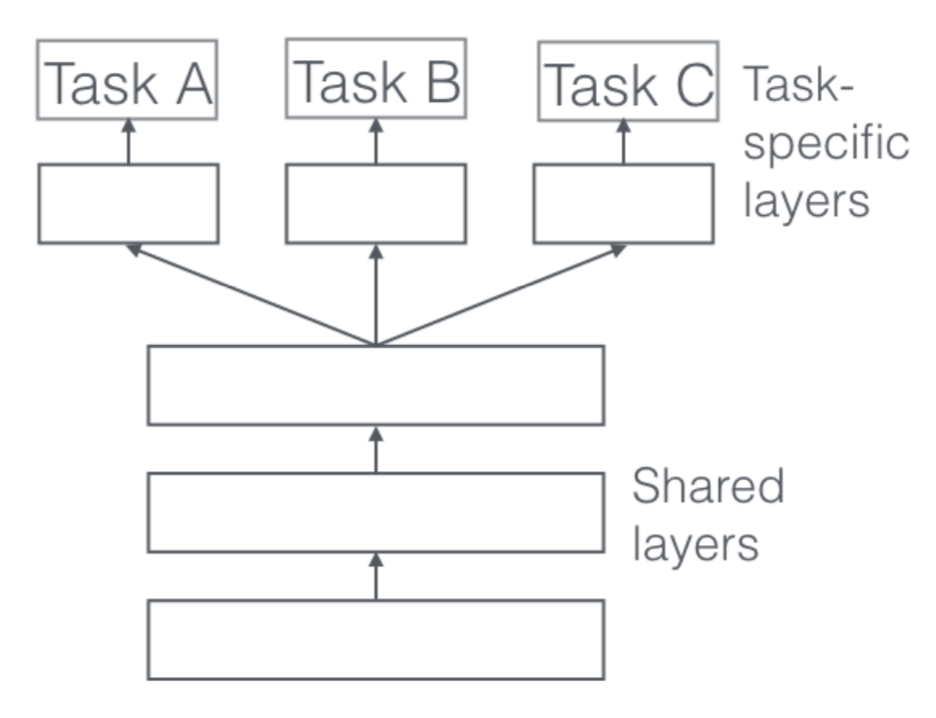
\includegraphics[width=.7\linewidth]{MTL_hard.png}
  \label{fig:sub1}
\end{subfigure}%
\begin{subfigure}{.5\textwidth}
  \centering
  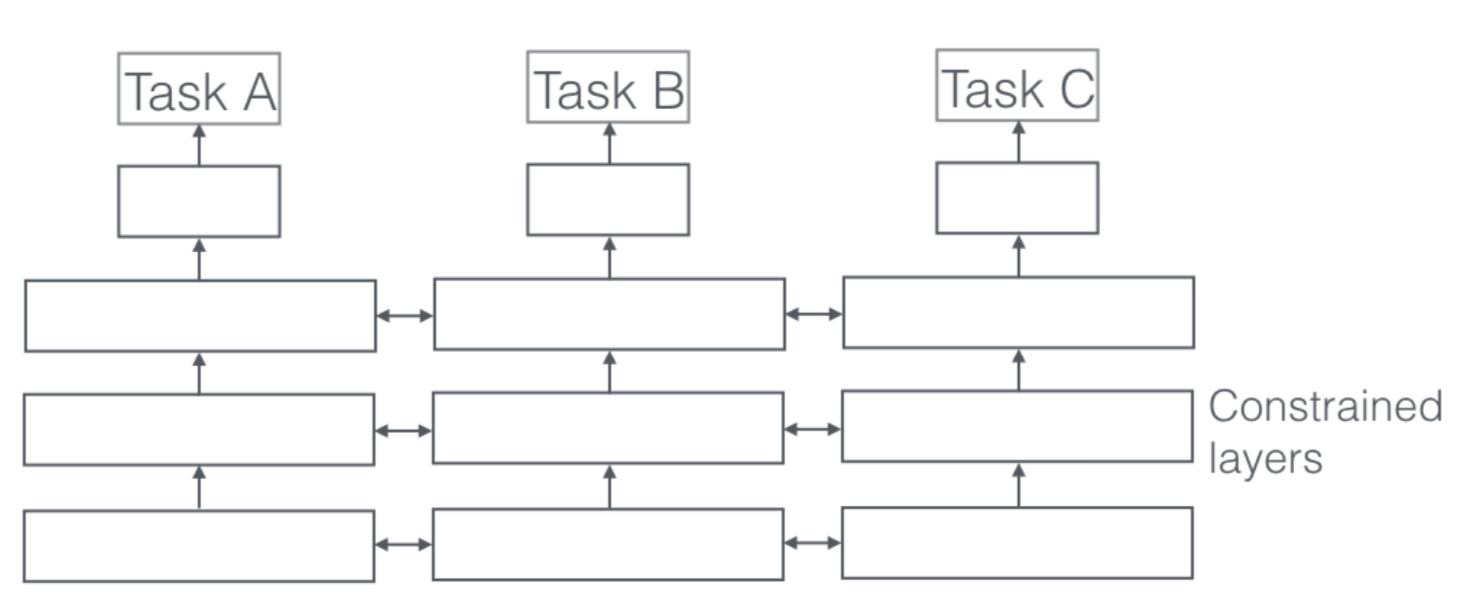
\includegraphics[width=1.2\linewidth]{MTL_soft}
  \label{fig:sub2}
\end{subfigure}
\caption{Hard parameter sharing, on the left, and soft parameter sharing, on the right, for multi-task learning in deep neural networks.}
\label{fig:test}
\end{figure}

As already mentioned, soft and hard parameters sharing are the two main used MTL methods in deep learning. Despite this, many works tried to develop better mechanisms for MTL in deep neural networks. Among them we can mention deep relationship networks \cite{NIPS2017_6757}, fully-adaptive feature sharing \cite{fullyadaptive}, cross-stitch networks \cite{crossstichnet}, low supervision \cite{sogaard-goldberg-2016-deep}, joint many-task model \cite{hashimoto-etal-2017-joint}, weighting losses with uncertainty \cite{Kendall}, tensor factorization for MTL \cite{Yang2017DeepMR} and, finally, sluice networks \cite{Ruder2017SluiceNL}.

\section{Gaussian Process for Hyper-parameters Tuning of the Models}
\label{sec:gaussianprocess}
% todo: integrate
% todo: read again
% todo: images
% todo: fix mathematical formalization (???)
In Section~\ref{sec:singletaskNN} and Section~\ref{sec:MTLsection} we
described the theoretical aspects of training single-task and multi-task neural networks. In practical terms, due to the
growing complexity of deep learning models, working with neural networks
involves a proper choice of many hyperparameters, such as the shape of
the network architecture, the learning rate, or the regularizer weight
decay. Over the years, many hyper-parameters optimization algorithms were
proposed. Among this, grid and random search \cite{BergstraB12} are significant examples. A more sophisticated model could be exploiting Bayesian optimization
and use it to choose the best hyper-parameters for a given model
\cite{SnoekGP}. In general, optimizers aim to minimize (or
maximize) a scoring function respect its hyper-parameters, given
$\mathcal{X}$ the set of hyper-parameters and $f(x)$ the scoring function of interest
(i.e., auPRC, auROC, rmse, binary loss etc.) we have: 
\[ 
x^* =  \argmin_{x \in \mathcal{X}} f(x) 
\]
the main difference between Bayesian optimization in comparison with more
traditional approaches is that Bayesian optimization chooses the next
hyper-parameters set in an informed way. It keeps track of past evaluations
that use to build a probabilistic model called \emph{surrogate function}. This function is often built using a Gaussian process. That is, in every
iteration the surrogate function is updated selecting, with a particular
\emph{selection function} (i.e., Expected Improvement function), and
evaluating a new set of hyper-parameters. On the one hand, Bayesian methods
take more time smartly choosing the next set of hyper-parameters. On the other hand, they make few iterations in total compared to grid and random search. 
Recently Keras developer has released a new hyperparameter optimizer
open-source library called Keras-tuner \footnote{Available on GitHub:
\url{https://github.com/keras-team/keras-tuner}}
\cite{omalley2019kerastuner}. It contains, among many others, an
implementation of Bayesian optimization\footnote{Documentation available
at: \url{https://keras-team.github.io/keras-tuner/documentation/tuners/}}.

\section{Evaluation Metrics} \label{sec:methods_metrics}
In this section the principal evaluation metrics used in this work are described. 
In Section~\ref{sec:singletaskNN} we described Stochastic Gradient Descend algorithm. In order to update the parameters of the network in Equation~\ref{eq:sgd} we have seen that we need to calculate the derivative of a convex loss function $\ell(.)$ with respect to the weights. In this work, in order to train both single and multi-tasks neural networks, we utilized a well-known loss function, often used in binary classification, called \emph{binary cross-entropy}. Given $t \in \{0, 1\}$, the true binary label of a sample, and $s \in [0\..1]$, the probability score given by a predictor, we define binary cross-entropy as:
\begin{equation}
    \ell(t, s) = -t\log(s) - (1 - t)\log(1 - s)
\end{equation}
In order to evaluate the performance of the models, many metrics can be used. Despite its simplicity, one of the most popular is \emph{Accuracy} defined as the proportion of the correct respect the total number of sample
\begin{equation}
    \textrm{accuracy} = \frac{\#\{\textrm{correct samples}\}}{\#\{\textrm{total samples}\}}
\end{equation}
It is easy to notice that the main drawback of accuracy is that, with an unbalanced dataset, we can achieve misleading higher values. Fortunately, during the years, more stable performance evaluation metrics were introduced in order to overcome accuracy disadvantages. In the contest of binary classification, before describing these new metrics, we must introduce four classification terms: 
\begin{itemize}
\item \emph{True Positive} (TP): samples classified as positive where also the actual value are positive;
\item \emph{False Positive} (FP): samples classified as positive where the actual values are negative;
\item \emph{True Negative} (TN): samples classified as negative where also the actual values are negative;
\item \emph{False Negative} (FN): samples classified as negative where the actual values are positive.
\end{itemize}
Of course, a good model aims to have a very high rate of true positive and true negative. From this point of view, to evaluate the goodness of a model, we can use \emph{precision} and \emph{recall}. Precision evaluate the ability of a model to classify relevant results correctly 
\begin{equation}
    \textrm{precision} = \frac{\textrm{TP}}{\textrm{TP}+\textrm{FP}}
\end{equation}
recall, instead, is the percentage of total relevant results correctly classified by the algorithm 
\begin{equation}
    \textrm{recall} = \frac{\textrm{TP}}{\textrm{TP}+\textrm{FN}}
\end{equation}
this two metrics are often put together computing the harmonic mean between them, obtaining a new metric called \emph{F1-score}:
\begin{equation}
    \textrm{F1-score} = 2 \cdot \frac{\textrm{precision} \cdot \textrm{recall}}{\textrm{precision}+\textrm{recall}}
\end{equation}
Finally, we describe the two main metrics used to evaluate the performance of the models used in this work: \emph{Area Under the Receiver Operating Characteristics} (auROC) and \emph{Area Under the Precision-Recall Curve} (auPRC). 
The auROC is computed plotting the ROC curve with Recall on y-axis against False Positive Rate (FPS) on x-axis and calculating the area under it.  Similarly, auPRC is computed plotting precision on y-axis against recall on x-axis and calculating the area under it. Since both precision and recall does not consider true negative sample, auPRC is used when having good performance on negative example are not extremely important. 